% Regression: main ink crosses two background runs; the second reuses the hook.
\documentclass[tikz,border=2pt]{standalone}
\usepackage{tikz}
\usetikzlibrary{backgrounds}
\begin{document}
\tikzset{every on background layer/.style={color=red,line width=1pt}}
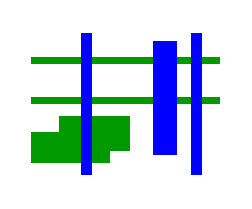
\begin{tikzpicture}[color=blue,line width=4pt]
  \draw (.7,-.15) -- (.7,1.65);
  \begin{scope}[color=magenta,line width=6pt,
                on background layer={color=green!60!black,line width=2.5pt}]
    \fill (0,0) rectangle (1,.4);
    \draw (0,1.3) -- (2.4,1.3);
  \end{scope}
  \fill (1.55,.1) rectangle (1.85,1.55);
  \begin{scope}[on background layer,color=magenta,line width=6pt]
    \fill (.35,.15) rectangle (1.25,.6);
    \draw (0,.8) -- (2.4,.8);
  \end{scope}
  \draw (2.1,-.15) -- (2.1,1.65);
\end{tikzpicture}
\end{document}
